\title{Лекция 2\\Базовый язык представления знаний}   
\author[]{Шункевич Д.В.}
\institute[]{Белорусский государственный университет информатики и радиоэлектроники}

\begin{frame}
	\titlepage
\end{frame}

\begin{frame}{\\Содержание лекции}
	\topline
	\justifying
	\begin{itemize}
	\item основные положения базового языка представления знаний в интеллектуальных системах – SC-кода
	\item алфавит, синтаксис, базовая денотационная семантика SC-кода
	\item синтаксическая и семантическая классификация sc-элементов
	\end{itemize}
\end{frame}

\begin{frame}{\\*}
	\begin{SCn}
		\scnheader{Sc-code} 
		\scnidtf{способ универсального смыслового представления (кодирования) информации в памяти компьютерных систем}
		\scnidtf{semantic computer code}
		\scnrelfrom{примечание}{SC-code основан на \textit{теории графов} (синтаксис) и \textit{теории множеств} (семантика), что обеспечивает универсальность и унифицированность (единообразие) представления информации, удобство машинной обработки и восприятия человеком}
	\end{SCn}
\end{frame}

\begin{frame}{\\*}
	\begin{SCn}
		\scnheader{двоичное кодирование}
			\begin{scnrelfromset}{характеристики}
				\scnitem {алфавит \{0, 1\}}
				\scnitem {не удобен для человека}
				\scnitem {удобен для обработки в компьютере}
				\scnitem {нельзя понять информацию без контекста}
				\scnitem {легко реализовать}
			\end{scnrelfromset}
		\scnheader{SC-code}
			\begin{scnrelfromset}{характеристики}
				\scnitem {базовый алфавит состоит из 5 элементов}
				\scnitem {удобен для человека}
				\scnitem {удобен для обработки в компьютере}
				\scnitem {обладает «осмысленностью»}
			\end{scnrelfromset}
	\end{SCn}
\end{frame}

\begin{frame}{\\*}
	\begin{SCn}
		\scnheader{SC-code}
		\scnidtf{абстрактный язык, который находится в памяти компьютерной системы}
		\scnrelfrom{примечание}{С помощью SC-кода можно описывать базы знаний, решатели задач и интерфейс интеллектуальной системы. SC-code является абстрактным языком, но его можно визуализировать в различных формах}
		\scnheader{формы внешнего представления SC-кода}
		\begin{scnrelfromset}{разбиение}
			\scnitem {SCs-code (текстовый линейный)}
			\scnitem {SCn-code (гипертекстовый)}
			\scnitem {SCg-code (графический)}
		\end{scnrelfromset}
	\end{SCn}
\end{frame}

\begin{frame}{\\*}
	\begin{columns}[T,onlytextwidth]
		\begin{column}{0.4\textwidth}
				\begin{SCn}
					\scnheader{SCs}
					\scnidtf{Semantic Code string}
					\scnidtf{язык линейного представления знаний}
					\scnheader{SCn}
					\scnidtf{Semantic Code natural}
					\scnidtf{язык структурированного представления знаний}
					\scnheader{SCg}
					\scnidtf{Semantic Code graphic}
					\scnidtf{язык графического представления знаний}
				\end{SCn}
		\end{column}
		\begin{column}{0.5\textwidth}
			\vspace{10mm}
			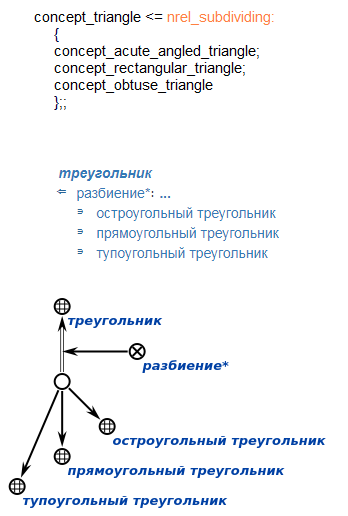
\includegraphics[width=50mm]{./part1/pictures/ostis-basics-1.png}
		\end{column}
	\end{columns}
\end{frame}

\begin{frame}{\\*}
	\begin{SCn}
		\scnheader{SC-code}
		\scnrelfrom{эпиграф}{Информация содержится не в самих знаках, а в конфигурации связей между ними}
		\scniselement{абстрактный язык}
		\scniselement{графовый язык}
		\begin{scnrelfromset}{основные положения}
			\scnitem{знаки сущностей --  синтаксически элементарные (атомарные) фрагменты sc-текстов, такие знаки не имеют внутренней структуры}
			\scnitem{информационные конструкции, не являющиеся sc-текстами, могут быть включены в базу знаний в виде файлов}
			\scnitem{тексты sc-кода имеют нелинейную (графовую) структуру, так как каждый знак сущности входит в базу знаний однократно и имеет неограниченное количество связей с другими знаками сущностей}
			\scnitem{...}
		\end{scnrelfromset}
	\end{SCn}
\end{frame}

\begin{frame}{\\*}
	\begin{SCn}
		\scnheader{SC-code}
		\begin{scnrelfromset}{основные положения}
			\scnitem{база знаний (в виде текста SC-кода) является графовой структурой, алфавит элементов которой включает в себя множество узлов, ребер, дуг, базовых дуг, а также множество специальных узлов, каждый из которых имеет содержимое, являющееся файлом, хранящимся в памяти интеллектуальной компьютерной системы}
			\scnitem{структурная особенность графовой структуры базы знаний заключается в том, что ее дуги и ребра могут связывать не только узел с узлом, но и узел с ребром или дугой, ребро или дугу с другим ребром или дугой}
			\scnitem{отсутствие синонимии осуществляется благодаря склеиванию (отождествлению) одинаковых sc-элементов}
			\scnitem{sc-узлы, sc-ребра и sc-дуги являются обозначениями различных сущностей}
		\end{scnrelfromset}
	\end{SCn}
\end{frame}

\begin{frame}{\\*}
	\begin{SCn}
		\scnheader{ребро}
			\scnrelfrom{обозначение}{бинарная неориентированная связка}
		\scnheader{дуга}
			\scnrelfrom{обозначение}{бинарная ориентированная связка}
		\scnheader{базовая дуга}
			\scnrelfrom{обозначение}{связь между узлом (обозначающим некоторое множество элементов) и одним из элементов, который принадлежит указанному множеству}
		\scnheader{узел с содержимым}
			\scnrelfrom{обозначение}{файл}
	\end{SCn}
\end{frame}

\begin{frame}{\\*}
	\begin{SCn}
		\scnheader{узел без содержимого}
		\scnrelfrom{обозначение}{материальный объект, первичный абстрактный
		объект (например, число, точка в некотором абстрактном пространстве), какая-либо бинарную связь, множество и т.д.}
		\scnheader{sc-сущности}
		\begin{scnrelfromset}{разбиение}
			\scnitem{постоянные (существуют всегда)}
			\scnitem{временные (им соотвествует отрезок времени их существования)}
			\scnitem{константные (конкретные)}
			\scnitem{переменные (произвольные)}
		\end{scnrelfromset}
	\end{SCn}
\end{frame}

\begin{frame}{\\*}
	\begin{SCn}
		
	\end{SCn}
\end{frame}




